% *******************************************************************************
% * Copyright (c) 2007 by Elexis
% * All rights reserved. This document and the accompanying materials
% * are made available under the terms of the Eclipse Public License v1.0
% * which accompanies this distribution, and is available at
% * http://www.eclipse.org/legal/epl-v10.html
% *
% *  $Id: icpc-plugin.tex 1951 2007-02-26 09:34:52Z rgw_ch $
% *******************************************************************************
% !Mode:: "TeX:UTF-8" (encoding info for WinEdt)

\section{CISP}
Le Plugin CISP intègre le \textit{International Code for Primary Care} Version 2 dans Elexis, mais permet indépendamment de cela et basé sur les problèmes du patient à établir un doisser électronique structuré.
\index{dossier électronique orienté selon les problèmes}
\index{problème}
\subsection{liste des problèmes}
\begin{wrapfigure}{r}{6cm}
  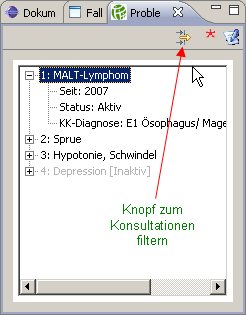
\includegraphics{images/problemliste1}
  \caption{Problemliste}\label{fig:problemliste}
\end{wrapfigure}

La liste des problèmes (Fig. \ref{fig:problemliste}) vous permet d'introduire les problèmes (aussi dénominés épisodes) comme texte libre et de leur attribuer un numéro. Lors de la mise en page il seront automatiquement ordonnés selon ces numéros. Si vous voulez donner à un problème une priorité mineure il suffit de lui attribuer un noméro plus bas. Si vous voulez par contre marquer un problème comme 'sous-problème' d'un autre, vous pouvez lui attribuer un numéro avec un point: Problème 2.1 sera automatiquement attribué au problème 2 et affiché entre 2 et 3.

Pour introduire un nouveau problème cliquez sur le symbole de l'étoile qui se trouve tout en haut de la 'view'. Pour effacer un problème veuillez cliquer dessus avec la touche droite et choisissez \textit{effacer}. Pour modifier les propriétés d'un problème déjà introduit veuillez cliquer sur le symbol 'modifier'.

Un problème peut avoir plusieur propriétés différentes : par ex. une date de début, un status (actif ou inactif) et un diagnostic qui sera transmis à l'assureur (sur la facture). Ces propriétés seront affichées lorsque vous cliquez sur le petit signe + qui se trouve à gauche à côté du titre. Pour marquer l'état actif ou inactif d'un problème veuillez cliquer dessus avec la touche droite et choisissez le réglage corréspondant dans le menu contextuel.

Pour attribuer à un problème un diagnostic qui sera transmis à l'assureur  (il s'agit du diagnostic qui apparaîtera plustard sur la facture), vous pouvez tirer simplement un tel diagnostic depuis une liste des diagnostics (par exemple depuis la fenêtre du traitement etc) sur le problème concerné.

\begin{figure}[ht]
    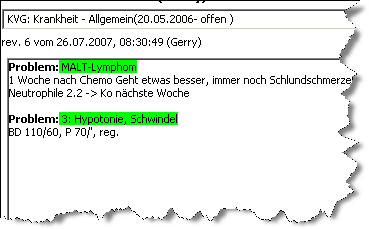
\includegraphics{images/problemliste2}
    \caption{Problem in Konsultationstext}
    \label{fig:problemliste2}
\end{figure}
Pour traiter un problème explicitement dans une consultation, veuillez le tirer avec la souris depuis la liste des problèmes dans la fenêtre des consultations. (Fig. \ref{fig:problemliste2}).

Si vous travaillez de façon conséquente avec la liste des problèmes vous allez trouver un gain supplémentaire : Si vous fixez le bouton 'filtrer' dans la fenêtre du listing des problèmes (Fig. \ref{fig:problemliste}) apparaîteront dans la 'view' des consultations (\ref{view:konsultationen}; page \pageref{view:konsultationen} ff.) automatiquement toujours que les consultations qui concernent le problème actuellement en question.
\label{filter:problemliste}
\index{consultations!filtrer} \index{Filtre}Un clic sur un autre problème filtre la liste des consultations de nouveau. Un nouveau clic sur le bouton 'filtrer' libère ce bouton de sorte que de nouveau toutes les consultations seront affichées.

\subsection{Encounter}
Pour pouvoir utiliser le plugin de a CISP-2 vous avez besoin le Code CISP-2 lequel vous pouvez importer facilement. Puisqu'il faut une licence pour l'utilisation commerciale de la CISP-2 nous n'avons pas le droit d'intégrer directement le code CISP-2. Concernant la licence veuillez vous informer directement chez le concessionnaire de votre pays. (en Suisse : la SSMG evt plus tard OMFS= Organisation des médecins de famille Suisse) comment et sous quelles conditions vous pouvez vous procurer le code.
\subsubsection{Idée}
Avec la CISP-2 on a l'intention de pouvoir mieux représenter le travail du médecin de famille que ce qui est possible avec les codes de la CIM-10 ou avec le Tarmed (Tarification médicale Suisse ein vigueur depuis 2004). Il doit être possible de codifier des symptômes comme on les trouve dans le travail quotidien du médecin de premier recours comme par exemple \glqq ne se sent pas bien\grqq ou \glqq a peur d'avoir du cancer\grqq. Il doit aussi être possible de déclarer des actes comme \glqq je l'ai examiné, consulté et tranquilisé concernant ses craintes\grqq ou de poser le diagnostic  \glqq de bonne santé\grqq. Si on collectionne ces données de façon structurée on peut scientifiquement mieux aborder le travail du médecin de premier recours et le comparer et quantifier mieux qu'avec un autre système de codification. Pour cette raison il y a des assiciations des médecins de premier recours dans des différents pays qui ont beaucoup d'intérêt à utiliser la CISP-2 pour avoir accès à ces données et ceci spécifiquement avec le but d'avoir des preuves lorsqu'il s'agit de s'investir pour une politique qui soutient la médecine de premier recours. (Que le code ne soit pourtant pas accessible librement est probablement résultat d'un de ces loopings de la logique qui arrivent parfois lorsque la realpolitik "se charge" des bonnes idées...)
\subsubsection{Introduction}

La codification selon la CISP-2 se fait concrètement lorsque on arrive à un point d'intersection \textit{Encounter} qui n'est rien d'autre qu'un épisode de maladie (d'une problème comme mentionné plus haut) qui mêne à une consultation. (\ref{fig:encounter}).\\
\begin{wrapfigure}{l}{7cm}
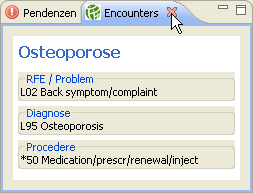
\includegraphics{images/encounter}
\caption{ICPC-Encounter}
\label{fig:encounter}
\end{wrapfigure}
Quand on se charge lors d'une consultation de deux problèmes on est face à exactement deux 'Encounters' et ceci même si on trouve en somme peut être 5 problèmes sur la liste des problèmes du patient.

Chaque Encounter est caractérisé par
\begin{itemize}
\item une raison (reason for encounter, rfe): Pour quelle raison le patient consulte ? Exemple: 'maux de tête'.
\item une appréciation (diagnostic). Exemple 'Migraine'.
\item un procédé. Exemple 'Medicament, conseils sur le style de vie'.
\end{itemize}

\bigskip

Im Elexis-ICPC-Plugin wird ein Encounter dadurch erstellt, dass ein Problem aus der Problemliste in ein Konsultationsfenster gezogen wird. Die genauere Definition des Encounters geschieht, indem man dann auf diesen Text doppelklickt. Das Encounter
-Fenster zeigt dann die Details des Encounters an. Durch Klick auf 'RFE' kann man aus der dann öffnenden Diagnosen-View den entsprechenden Code z.B. aus der ICPC-Komponente 1 (Symptom and Complaint component) einsetzen. Entsprechend wählt man für Diagnose einen Code aus der Komponente 7 (Diagnosis component) und für Procedere aus z.B. Komponente 3 (Medication, treatment, procedure component).
Genauere Informationen zur Anwendung der einzelnen ICPC-Komponenten finden Sie in der ICPC-Dokumentation. Weitere Informationen z.B. hier:

\href{http://www.primary-care.ch/pdf/2005/2005-10/2005-10-656.PDF}{http://www.primary-care.ch/pdf/2005/2005-10/2005-10-656.PDF}


\section{Sgam-xChange}
Sgam-xChange est un Plugin qui permet l'échange des données quelconques entre des systèmes qui contiennent un dossier électronique. Par exemple vous pouvez exporter de façon codifiée une feuille de labo ou même tout un dossier depuis votre programme vers un/e collègue qui pourra l'intégrer (importation) ensuite dans son dossier électronique - à condition que son programme soit apte au xchange.

xChange est un 'open standard', qui contient les élements suivants:
\begin{itemize}
 \item Le Transport-Format de fichier est nécessaire pour que les différents logiciels contenant le dossier électronique puissent  \textit{comprendre} les fichiers lesquels ils sauvegardent probablement d'une façon très différente.
\item Le Transport-Container définit une technologie de cryptage et de transfert pour que les données puissent être transportées de façon sécurisée de l'expéditeur au destinataire.
\end{itemize}
Pour faciliter l'implémentation de xChange à tout producteur de logiciel pour le cabinet médical le standard avait été limité consciemment aux élements les plus essentiels. Le standard est gratuitement mis à disposition à toute personne intéressée y inclus une application à titre exemplaire qui donne quelques instructions pour l'implémentation.

Sgam-xChange a été crée et sponsorisé par orde du groupe de travail  \href{http://www.sgam.ch/informatics}{Sgam.informatics} , qui est aussi l'interlocuteur pour des questions de licence.

\subsection{Conditions}


L'explication et la description du contexte technique vous trouvez ici. Cet article se limite à la description de l'implémentation de Sgam.xChange dans Elexis.

Pour pouvoir transporter des données depuis Elexis à l'aide de Sgam.xChange, vous avez besoin à part de Elexis et du Plugin Sgam.xChange (qui est intégré d'emblé dans Elexis), du programme de cryptage \href{http://www.gnupg.org}{GnuPG}.

 GnuPG est disponible gratuitement pour les principaux systèmes d'exploitation (Windows, Linux, Mac). Il s'agit d'un système de cryptage OpenSource qui existe depuis 1999 et qui jouit d'une excellente réputation. (Certains pays par contre l'interdisent car il ne peut même pas être cassées par les services secrets.) En Suisse l'utilisation est légale.
\subsection{Installation et  Configuration}

GPG peut être installé à n'importe quel endroit pourvu qu'Elexis est mis au courrant où il se trouve. Veuillez ouvrir pour cela dans le menu es muss dann lediglich an Elexis bekanntgemacht werden, wo es liegt. Öffnen Sie dazu im Menü \textit{Fichier-Paramètres} l'onglet \textit{xChange}:

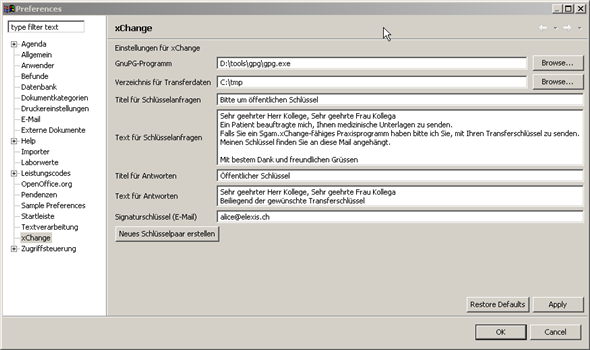
\includegraphics[width=3in]{images/xc1.png}
% xc1.png: 590x350 pixel, 96dpi, 15.61x9.26 cm, bb=0 0 442 262

Ensuite on peut procéder aux réglages suivants:
\begin{itemize}
 \item GnuPG-Programme: Le 'full path' à gpg.exe
\item Le répertoire pour les données de transfert: Un répertoire existant dans lequel xChange peut mettre en mémoir tampon des données.
\item Titre pour des demandes de clé: xChange peut générer automatiquement des e-mails pour demander la clé publique du correspondant. Ici vous pouvez introduire le titre souhaité pour un tel e-mail.
\item Texte pour des demandes de clé: Introduisez ici le texte que vous souhaitez mettre dans le e-mail de demande de clé.
\item Titre pour réponse: xChange peut aussi générer automatiquement un e-mail pour la réponse à une demande de clé. Veuillez introduire ici le titre d'un telle réponse.
\item Texte pour réponse: Le contenu du texte d'une réponse par e-mail.
 Clé de signature (E-Mail): Veuillez introduire ici la clé qui doit être utilisée de façon standardisée pour xChange. Souvent ça sera de toute façon votre seule clé. Veuillez introduir l'adresse e-mail à laquelle sera liée cette clé.

\item
\item Créer une nouvelle paire de clé:  . Si vous n'avez pas encore une clé-GPG vous pouvez créer une paire de clé en cliquant sur ce bouton. (Une paire de clé consiste en une clé privée qui est sécurisée par un mot de passe nécessaire pour signer et pour décrypter et une clé publique correspondante que vous pouvez donner à toute personne intéressée pour pouvoir crypter des messages que vous souhaitez envoyer ou pouvoir verifier leurs signatures lorsque vous recevez des messages.)
\end{itemize}

Après avoir pressé le bouton la fenêtre suivante s'ouvre:

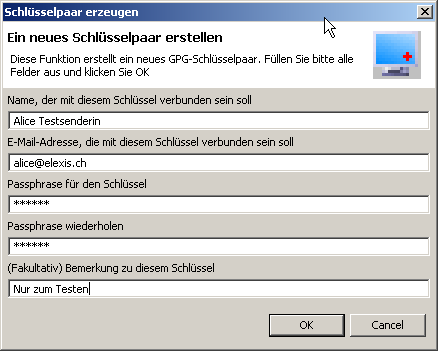
\includegraphics[width=3in]{images/xc2.png}
% xc2.png: 438x351 pixel, 96dpi, 11.59x9.29 cm, bb=0 0 328 263

Les instructions sont évidentes. Avec cette clé xChange va signer vos envois  et va essayer de décrypter les envois que vous recevez.
(Des explications plus détaillées vous trouverez \href{http://www.elexis.ch/jp/index.php?option=content&task=view&id=64}{ici})
\subsection{Exporter un dossier électronique}
Veuillez cliquer avec la touche droite sur l'inscription se trouvant dans le dossier électronique et choisissez  \textit{exporter dossier électronique}

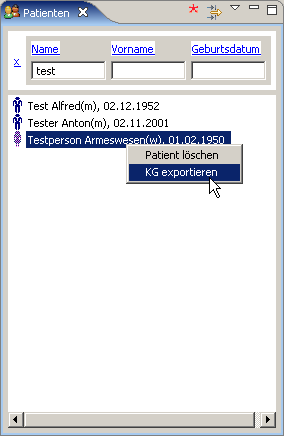
\includegraphics[width=3in]{images/xc3.png}
% xc3.png: 284x436 pixel, 96dpi, 7.51x11.53 cm, bb=0 0 213 327

 Le dialogue suivant apparaîtra:

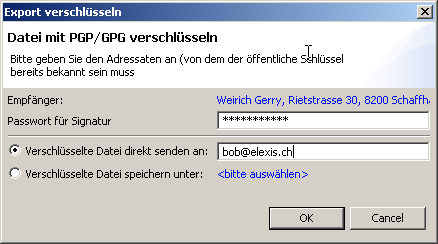
\includegraphics[width=3in]{images/xc4.png}
% xc4.png: 438x244 pixel, 96dpi, 11.59x6.46 cm, bb=0 0 328 183

Après avoir cliqué sur \textit{OK} le dossier électronique sera automatiquement crypté et envoyé vers le destinataire qui ne pourra le décrypter seulement avec sa clé mentionné en haut sous \textit{destinataire}.

\subsection{Du côté destinataire}
Du côté destinataire le e-mail sera reçu:

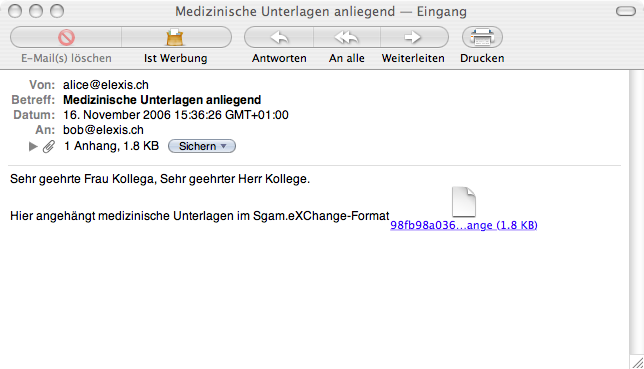
\includegraphics[width=3in]{images/import1.png}
% import1.png: 644x369 pixel, 72dpi, 22.72x13.02 cm, bb=0 0 644 369

La pièce jointe au mail sera le fichier xChange.

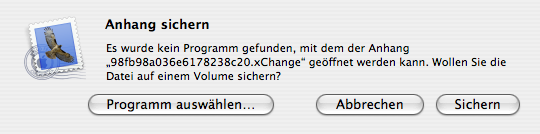
\includegraphics[width=3in]{images/import2.png}
% import2.png: 540x134 pixel, 72dpi, 19.05x4.73 cm, bb=0 0 540 134

Depuis le menu 'Fichier-Importation' le xChange fichier peut être sauvegardé et directement intégré dans Elexis.

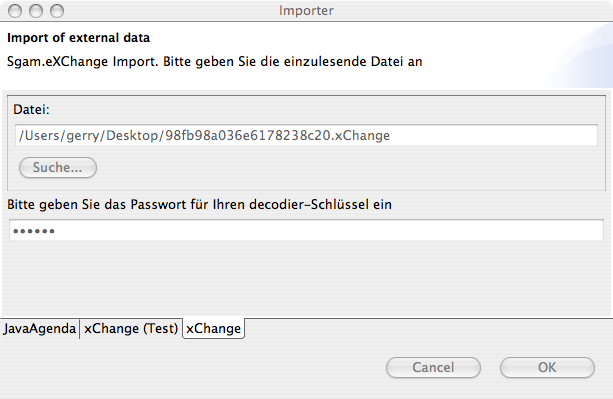
\includegraphics[width=3in]{images/import3.png}
% import3.png: 613x399 pixel, 72dpi, 21.63x14.08 cm, bb=0 0 613 399



Si vous détenez la clé correcte le dossier électronique sera importé directement dans votre logiciel. 

Concernant la stratégie de géstion des clés veuillez lire \href{http://www.elexis.ch/jp/index.php?option=content&task=view&id=64}{ici} les détails.

\section{Elexis-ebanking-Suisse}
Intégration du système suisse BVR/DTA pour paiement en monnaie scripturale. Ce Plugin fait partie de la distribution standard de Elexis. Lui-même ne contient pas de 'user fonctions' mais il doit pourtant être installé si d'autres Plugins veulent utiliser les fonctions pour le E-Banking. 